\subsection{Context and Motivations}
%
The choice of having a CarPal service per community (companies,
universities, etc.) comes from the need of having groups of people with
common travel patterns, habits, activities or even interests.  However
it's easy to see how such approach leads to the situation where two or
more different communities might be \emph{geographically overlapping},
\ie\ residing in the same area and \emph{not be aware of each other}
thus one not taking advantage of the other's free places. Often
companies are very close geographically and they have the same working
timetable. If, as intended, different companies have put in place
different CarPal communities, those possible matches will not be
taken into account.

As said in the introduction, any attempt of make different and
disconnected institutional, client-server based, Carpool services does
not foresee any form of service interconnection with the unpleasant
consequence of loosing potential matches between offers and requests
between users of different communities but living in the same region.
Very often the problem is not (only) technological: institutions do
not want to share their databases, or we don't trust the reputation
of other companies, or simply we want to travel with people of the
same enterprise.

In order to circumvent such limitation, communities can be
interconnected using our Arigatoni~\cite{CCL08} and
Synapse~\cite{LTVBCM09,LTB09} protocols developed in our team during
the Aeolus project.  Such meta-protocol allows a request to be routed
through multiple overlays, even using different routing algorithms,
thus increasing the success rate of every request. In case of
Arigatoni, communications and routing inter-overlays goes through a
broker-2-broker negotiation, where a broker is a special peer that can
be considered as the leader of the overlay \cite{LC07b}. In case of
Synapse, that represents an evolution of Arigatoni taking advantage of
the DHT technology of structured overlay networks, crossing overlays
is achieved through co-located nodes, represented by peers who are, by
user's choice, member of several communities.  Such nodes are able
themselves not only to query multiple communities in order to find a
match but also to replicate requests passing through them from one
network to another and to collect the multiple results. In the next
subsection we will briefly introduce the synapse protocol.


\subsection{Synapses in a nutshell}
%
The interconnection of overlay networks has been recently identified
as a promising model to cope with today's Internet issues such as
scalability, resource discovery, failure recovery or routing
efficiency, in particular in the context of information retrieval.
Some recent researches have focused on the design of mechanisms for
building bridges between heterogeneous overlay networks with the
purpose of improving cooperation between networks that have different
routing mechanisms, logical topologies and maintenance
policies. However we are still missing  more comprehensive approaches of such
interconnections for information retrieval and both quantitative and
experimental studies of its key metrics, such as satisfaction rate or
routing length.

Many disparate overlay networks may not only simultaneously co-exist
in the Internet but also compete for the same resources on shared
nodes and underlying network links. One of the problems of the overlay
networking area is how heterogeneous overlay networks may
\emph{interact} and \emph{cooperate} with each other. Overlay networks
are heterogeneous and basically unable to cooperate each other in an
effortless way, without merging, an operation which is very costly
since it not scalable and not suitable in many cases for security
reasons. However, in many situations, distinct overlay networks could
take advantage of cooperating for many purposes: collective
performance enhancement, larger shared information, better resistance
to loss of connectivity (network partitions), improved routing
performance in terms of delay, throughput and packets loss, by, for
instance, cooperative forwarding of flows.

As a basic example, let us consider two distant databases. One node of
the first database stores one $(key, value)$ pair which is searched by
a node of the second one. Without network cooperation those two nodes
will never communicate together. As another example, we have an
overlay network where a number of nodes got isolated by an overlay
failure, leading to a partition: if some or all of those nodes can be
reached via an alternative overlay, than the partition could be
recovered via an alternative routing.

In the context of large scale information retrieval, several overlays
may want to offer an aggregation of their information/data to their
potential common users without losing control of it.  Imagine two
companies wishing to share or aggregate information contained in their
distributed databases, obviously while keeping their proprietary
routing and their exclusive right to update it.  Finally, in terms of
fault-tolerance, cooperation can increase the availability of the
system, if one overlay becomes unavailable\,the global network will
only undergo partial failure as other distinct resources will be
usable.

We consider the tradeoff of having one \vs\ many overlays as a
conflict without a cause: having a single global overlay has many
obvious advantages and is the \textit{de facto} most natural solution,
but it appears unrealistic in the actual setting. In some optimistic
case, different overlays are suitable for collaboration by opening
their proprietary protocols in order to build an open standard; in
many other pessimistic cases, this opening is simply unrealistic for
many different reasons (backward compatibility, security, commercial,
practical, etc.). As such, studying protocols to interconnect
collaborative (or competitive) overlay networks is an interesting
research vein.

The main contribution of this research vein is to introduce, simulate
and experiment with \emph{Synapse} \cite{LTVBCM09}, a scalable
protocol for information retrieval over the inter-connection of
heterogeneous overlay networks. The protocol is based on co-located
nodes, also called \emph{synapses}, serving as low-cost natural
candidates for inter-overlay bridges. In the simplest case (where
overlays to be interconnected are ready to adapt their protocols to
the requirements of interconnection), every message received by a
co-located node can be forwarded to other overlays the node belongs
to. In other words, upon receipt of a search query, in addition to its
forwarding to the next hop in the current overlay (according to their
routing policy), the node can possibly start a new search, according
to some given strategy, in some or all other overlay networks it
belongs to. This obviously implies to providing a Time-To-Live value
and detection of already processed queries, to avoid infinite loop in
the networks, as in unstructured peer-to-peer systems.  Applications
of top of Synapse see those inter-overlay as a unique overlay.

We also study interconnection policies as the explicit possibility to
rely on \emph{social} based strategies to build these bridges between
distinct overlays; nodes can invite or can be invited. In case of
concurrent overlay networks, inter-overlay routing becomes harder, as
intra-overlays are provided as some black boxes: a \emph{control}
overlay-network made of co-located nodes maps one hashed key from one
overlay into the original key that, in turn, will be hashed and routed
in other overlays in which the co-located node belongs to. This extra
structure is unavoidable to route queries along closed overlays and to
prevent routing loops.

Our experiments and simulations show that a small number of
well-connected synapses is sufficient in order to achieve almost
exhaustive searches in a ``synapsed'' network of structured overlay
networks. We believe that Synapse can give an answer to circumventing
network partitions; the key points being that:
  %
   \begin{itemize}
   \item several logical links for one node leads to as many
     alternative physical routes through these overlay, and
  %
   \item a synapse can retrieve keys from overlays that it does not
     even know simply by forwarding their query to another synapse
     that, in turn, is better connected.
 \end{itemize}
%
 Those features are achieved in Synapse at the cost of some additional
 data structures and in an orthogonal way to ordinary techniques of
 caching and replication. Moreover, being a synapse can allow for the
 retrieval of extra information from many other overlays even if we
 are not connected with.  Finally, Synapse can either work with
 ``open'' overlays adapting their protocol to synapse interconnection
 requirements, or with ``closed'' overlays that will not accept any
 change to their protocol. Figure \ref{fig:example} shows how Synapse
 can give an answer in case of routing across differents
 intra-overlays and dealing with network partitions. For more details,
 see \cite{LTVBCM09}.



\begin{figure}[!t]
  \centering
  \mbox{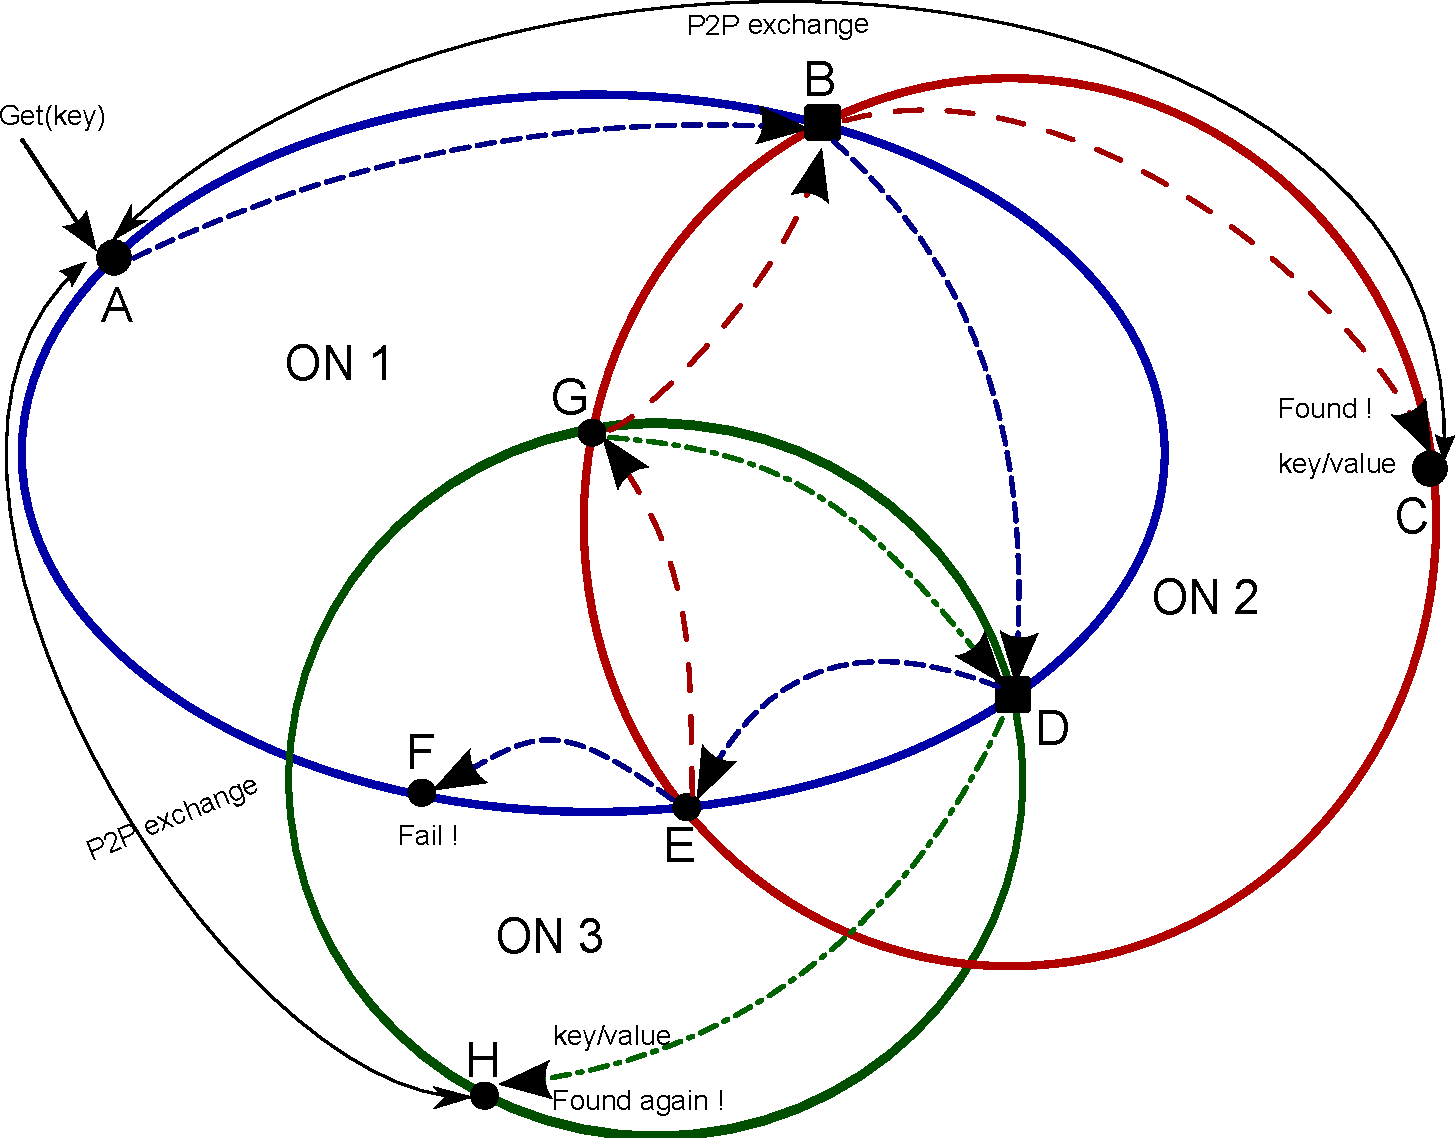
\includegraphics[width=0.4\columnwidth]{fig/GET_into_other_ON.pdf}\,\,
    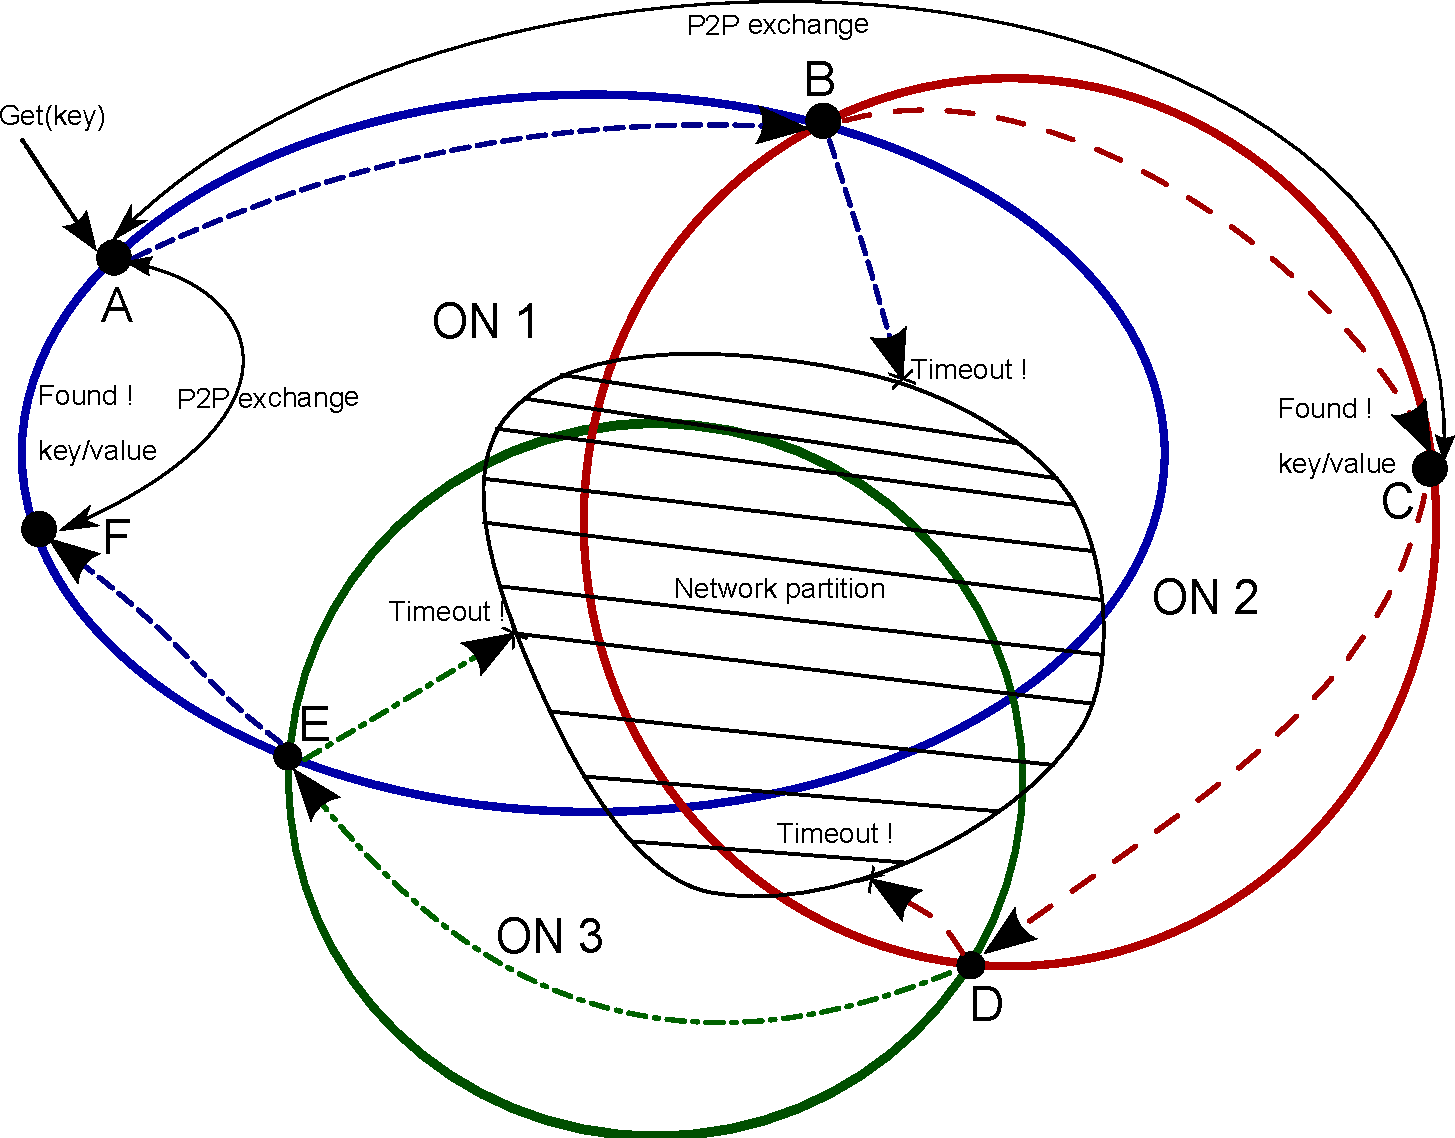
\includegraphics[width=0.4\columnwidth]{fig/ON_with_network_partition.pdf}}
  \caption{Routing across differents overlays and dealing with a network partition\label{fig:example}}
\end{figure}